% Chapter Template

\chapter{Chemogenetic Perturbation of Mouse Parietal Cortex} % Main chapter title

\label{Chapter3} 

One of the computational frameworks explaining how a neural circuit might implement evidence accumulation for decision making proposes a mechanism in which separate populations of neurons that modulate the net activity of the circuit in favor of (or against) a possible outcome of the decision. Inhibition plays a central role in these frameworks. For example, one class of models \parencite{Wang2002,Usher2001,Machens2005,Brown2001} suggests that inhibitory neurons mediate “competitive inhibition” between neuronal ensembles representing evidence in favor of a particular. Another class of decision making models \parencite{Ma2006,Beck2008} suggests that inhibitory neurons, alternatively, mediate global or “homeostatic inhibition” to normalize the responses of excitatory neurons in the population and prevent saturation. Although computational models involving inhibition are capable of recapitulating behavioral and neurophysiological results, \parencite{Usher2001,Wang2002,Machens2005,Beck2008,Wong2007,Wong2006} there is limited experimental evidence to support the computational roles of inhibitory neurons in perceptual evidence accumulation. An appealing possibility is that inhibitory neurons in the mouse posterior parietal cortex, a putative decision area, are involved in shaping evolving decisions.\par 
This chapter describes the approach to disrupting activity in mouse PPC in freely behaving animals and summarizes the behavioral impact of mouse PPC disruption. Silencing inhibitory neurons in mouse PPC significantly impaired the subjects' performance on the visual evidence accumulation task. These experiments also served as a means to test whether the behavioral paradigm engaged cortical machinery.
%----------------------------------------------------------------------------------------
%	SECTION 
%----------------------------------------------------------------------------------------
\section{Approach}
A chemogenetic approach called DREADD (Designer Receptor Exclusively Activated by Designer Drug, \textcite{Rogan2011}) was used to disrupt activity in mouse PPC (Figure \ref{fig:dreaddstrategy}). The DREADD approach was favored over other pharmacological methods such as muscimol because it offered a minimally invasive approach to reversibly perturbing neural activity. DREADDs also offers greater target specificity than muscimol, as it incorporates a fluorescent label which indicates where in the brain the receptors are expressed, and where the DREADD agonist (Clozapine-N-Oxide, CNO) will likely act.\par 

To target inhibitory neurons, I used a transgenic mouse line expressing Cre-recombinase in Gad2-positive (Gad2+) neurons, in combination with a Cre-dependent virus (AAV8-DIO-hSyn-hM4Di-mCherry) carrying the inhibitory DREADD receptor (hM4Di). Standard virus injection was used to introduce the DREADD receptor, bilaterally (Figure \ref{fig:dreaddexpression}) into the published stereotactic mouse PPC coordinates (2mm posterior and 1.7mm lateral from bregma, \textcite{Harvey2012}). Injection of the virus into mouse PPC restricts expression of the inhibitory DREADD to Gad2+ interneurons. Full expression took approximately 3-4 weeks from the date of injection. During this time the mice were allowed to recover and begin training on the task. The manipulation experiments were started once the mice acquired the task (approximately 6-8 weeks).The DREADD is activated by a pharmacologically inert designer drug, CNO (Clozapine-N-Oxide), which binds to the exogenous receptor, and in the case of the inhibibitory DREADD, hM4Di, suppresses neural activity. Before the start of a given session, we administered either saline (0.9\%) or CNO (2 mg/kg) via intraperitoneal injection.
\begin{figure}
  \centering
  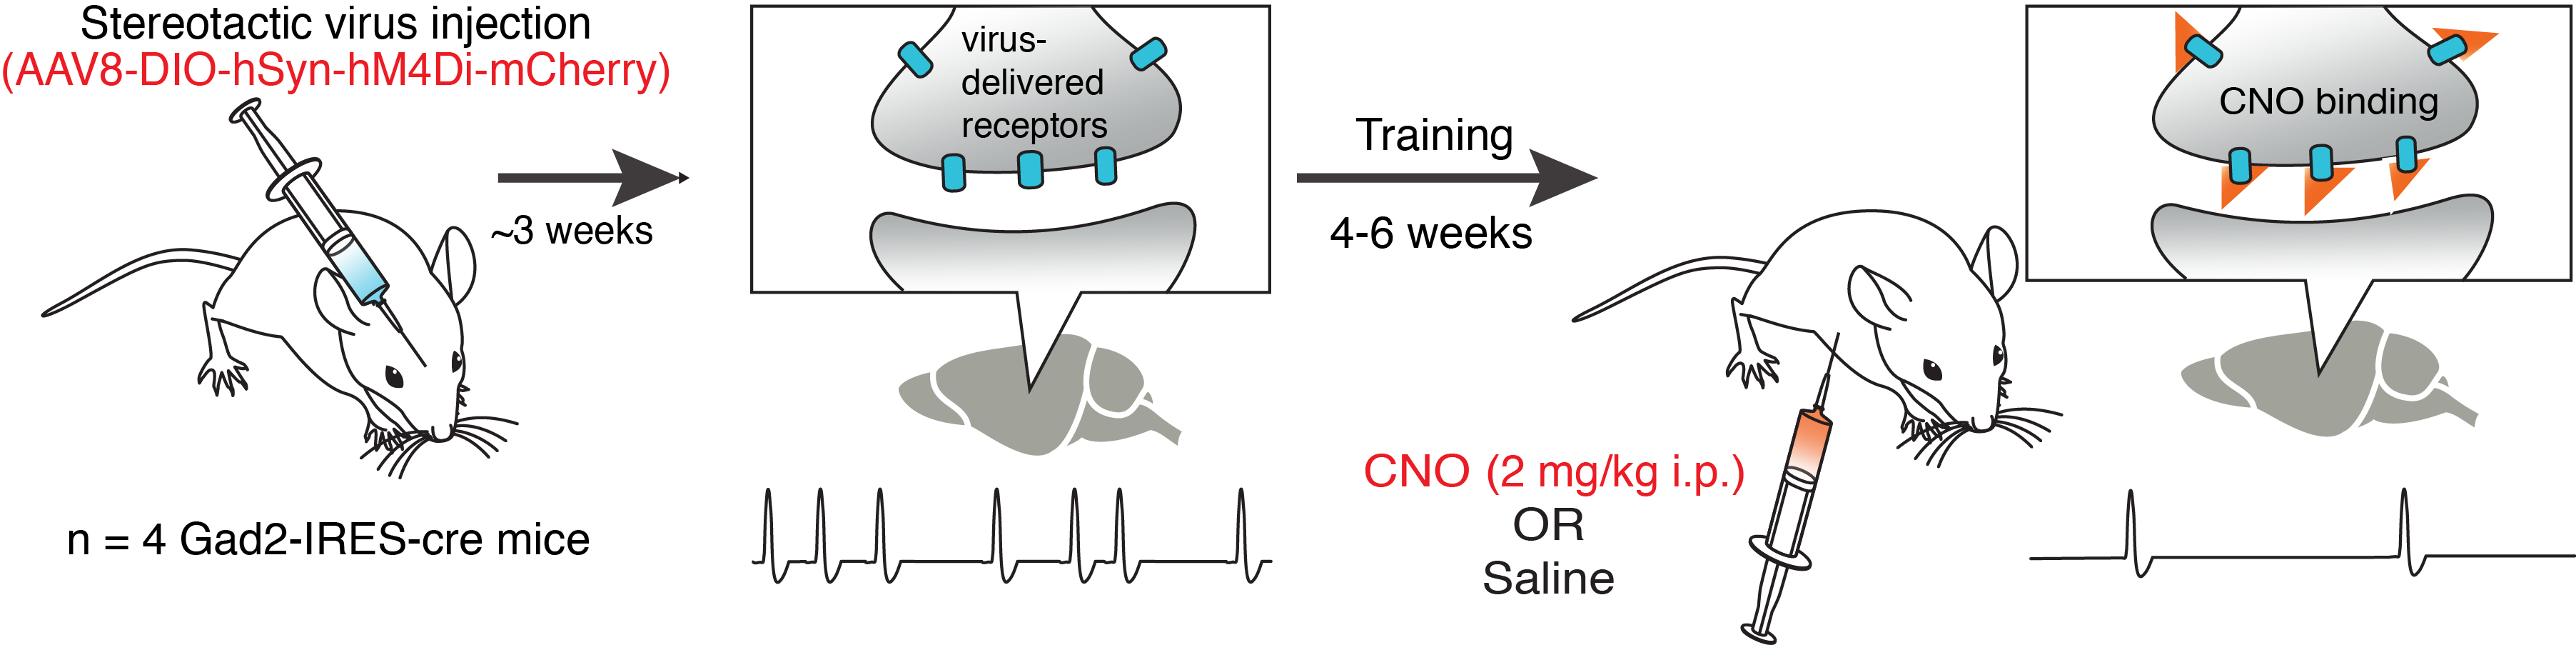
\includegraphics[width=\textwidth]{Figures/chapter3/DREADD_strategy.png}
  \caption[Strategy for Chemogenetic Manipulation of PPC]{\textbf{Strategy for Chemogenetic Manipulation of PPC.} Mice are injected with virus (AAV8-DIO-hSyn-hM4Di-mCherry) to express DREADD in PPC. Once the animals have acquired the decision task, they are given intraperitoneal injection of CNO or saline. Administration of CNO, activates the DREADD and reduces activity in cells expressing the receptor.}
   \label{fig:dreaddstrategy}
\end{figure}
\begin{figure}
  \centering
  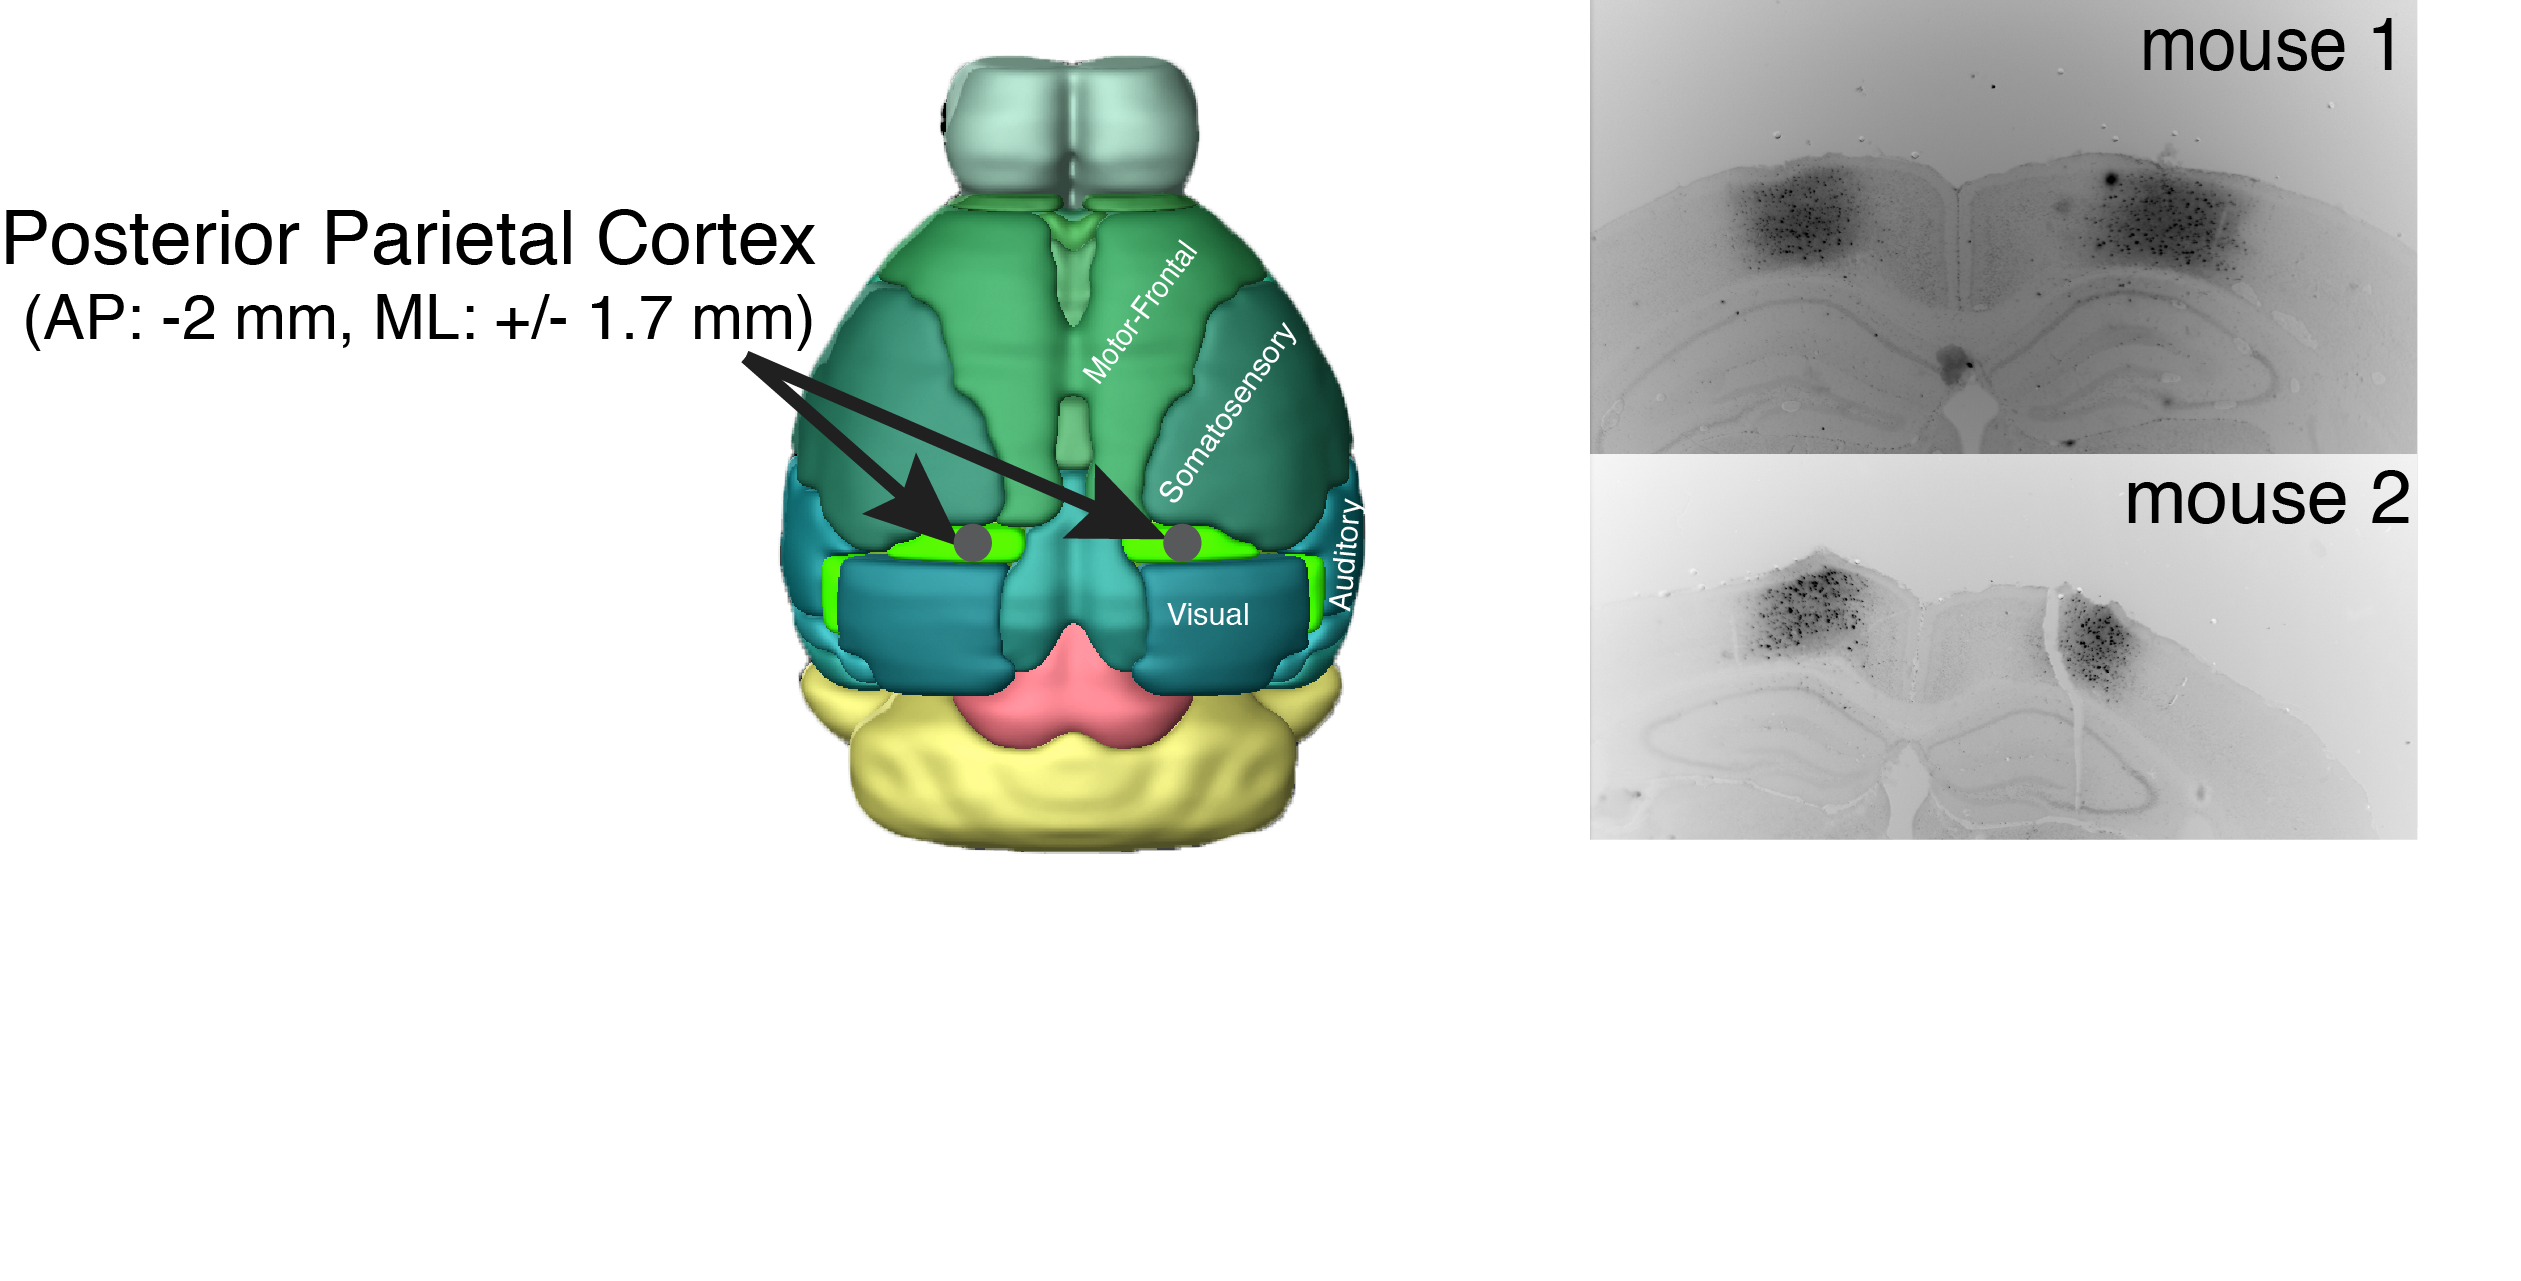
\includegraphics[width=\textwidth]{Figures/chapter3/DREADD_expression.png}
  \caption[Expression of inhibitory DREADD (hM4Di) in Gad+ neurons in PPC]{\textbf{Expression of inhibitory DREADD (hM4Di) in Gad+ neurons in PPC.} Fluorescence image of hM4Di-mCherry expression in mouse PPC for two example animals.}
   \label{fig:dreaddexpression}
\end{figure}
%----------------------------------------------------------------------------------------
%	SECTION 
%----------------------------------------------------------------------------------------
\section{DREADD silencing of PPC inhibitory neurons disrupts psychophysical performance}
Psychophysical performance of the mice expressing the DREADD receptor was reduced on CNO-treated sessions compared to saline control sessions (Figure \ref{fig:dreaddallmice}). The subjects' performance was quantified by estimating the slope of the psychometric curve function, which was fit with a cumulative Normal distribution (Psignifit). The width of the Gaussian ($\sigma$) reflects the inverse of the slope of the psychometric function and is related to the subject's sensitivity. Intuitively, the narrower the width of the Gaussian, the steeper the slope and the better the psychophysical performance. Conversely, the wider the Gaussian, the shallower the slope and the poorer the psychophysical performance. Across mice in this study, the slope of the psychometric function was much shallower on CNO treatment sessions compared to saline control sessions (Figure \ref{fig:dreaddallmice}c).\par 

Because the mice in Figure \ref{fig:dreaddallmice} were not trained to asymptotic performance before DREADD manipulation experiments, one concern is that the fit of the psychometric curve might yield poor estimates of the slope. Hence, performance was also quantified by estimating \emph{d'} (Equation \ref{dprime}), which is a signal detection theory index that quantifies the separation between the means of a signal and noise distribution \parencite{Macmillian,Green1989}.\emph{d'} is calculated according to the following equations:
\begin{equation}
\begin{aligned}	
    \centering
	d' &= \frac{\mu_H  - \mu_L}{\sqrt{0.5(\sigma^2_H + \sigma^2_L)}} \\
    d' &= Z(hit \: rate) - Z(false \: alarm)
\end{aligned}
\label{dprime}
\end{equation}
where $\mu$ and $\sigma$ represent the mean and the standard deviations of the high-rate (H) and low-rate (L) distributions; Z is the inverse cumulative Normal distribution. Intuitively, the higher the \emph{d'}, the better the psychophysical performance. Consistent with the estimates of the psychometric curve slope, \emph{d'} index was lower on CNO sessions compared to saline control sessions Figure \ref{fig:dreaddallmice}e.\par
\begin{figure}
  \centering
  	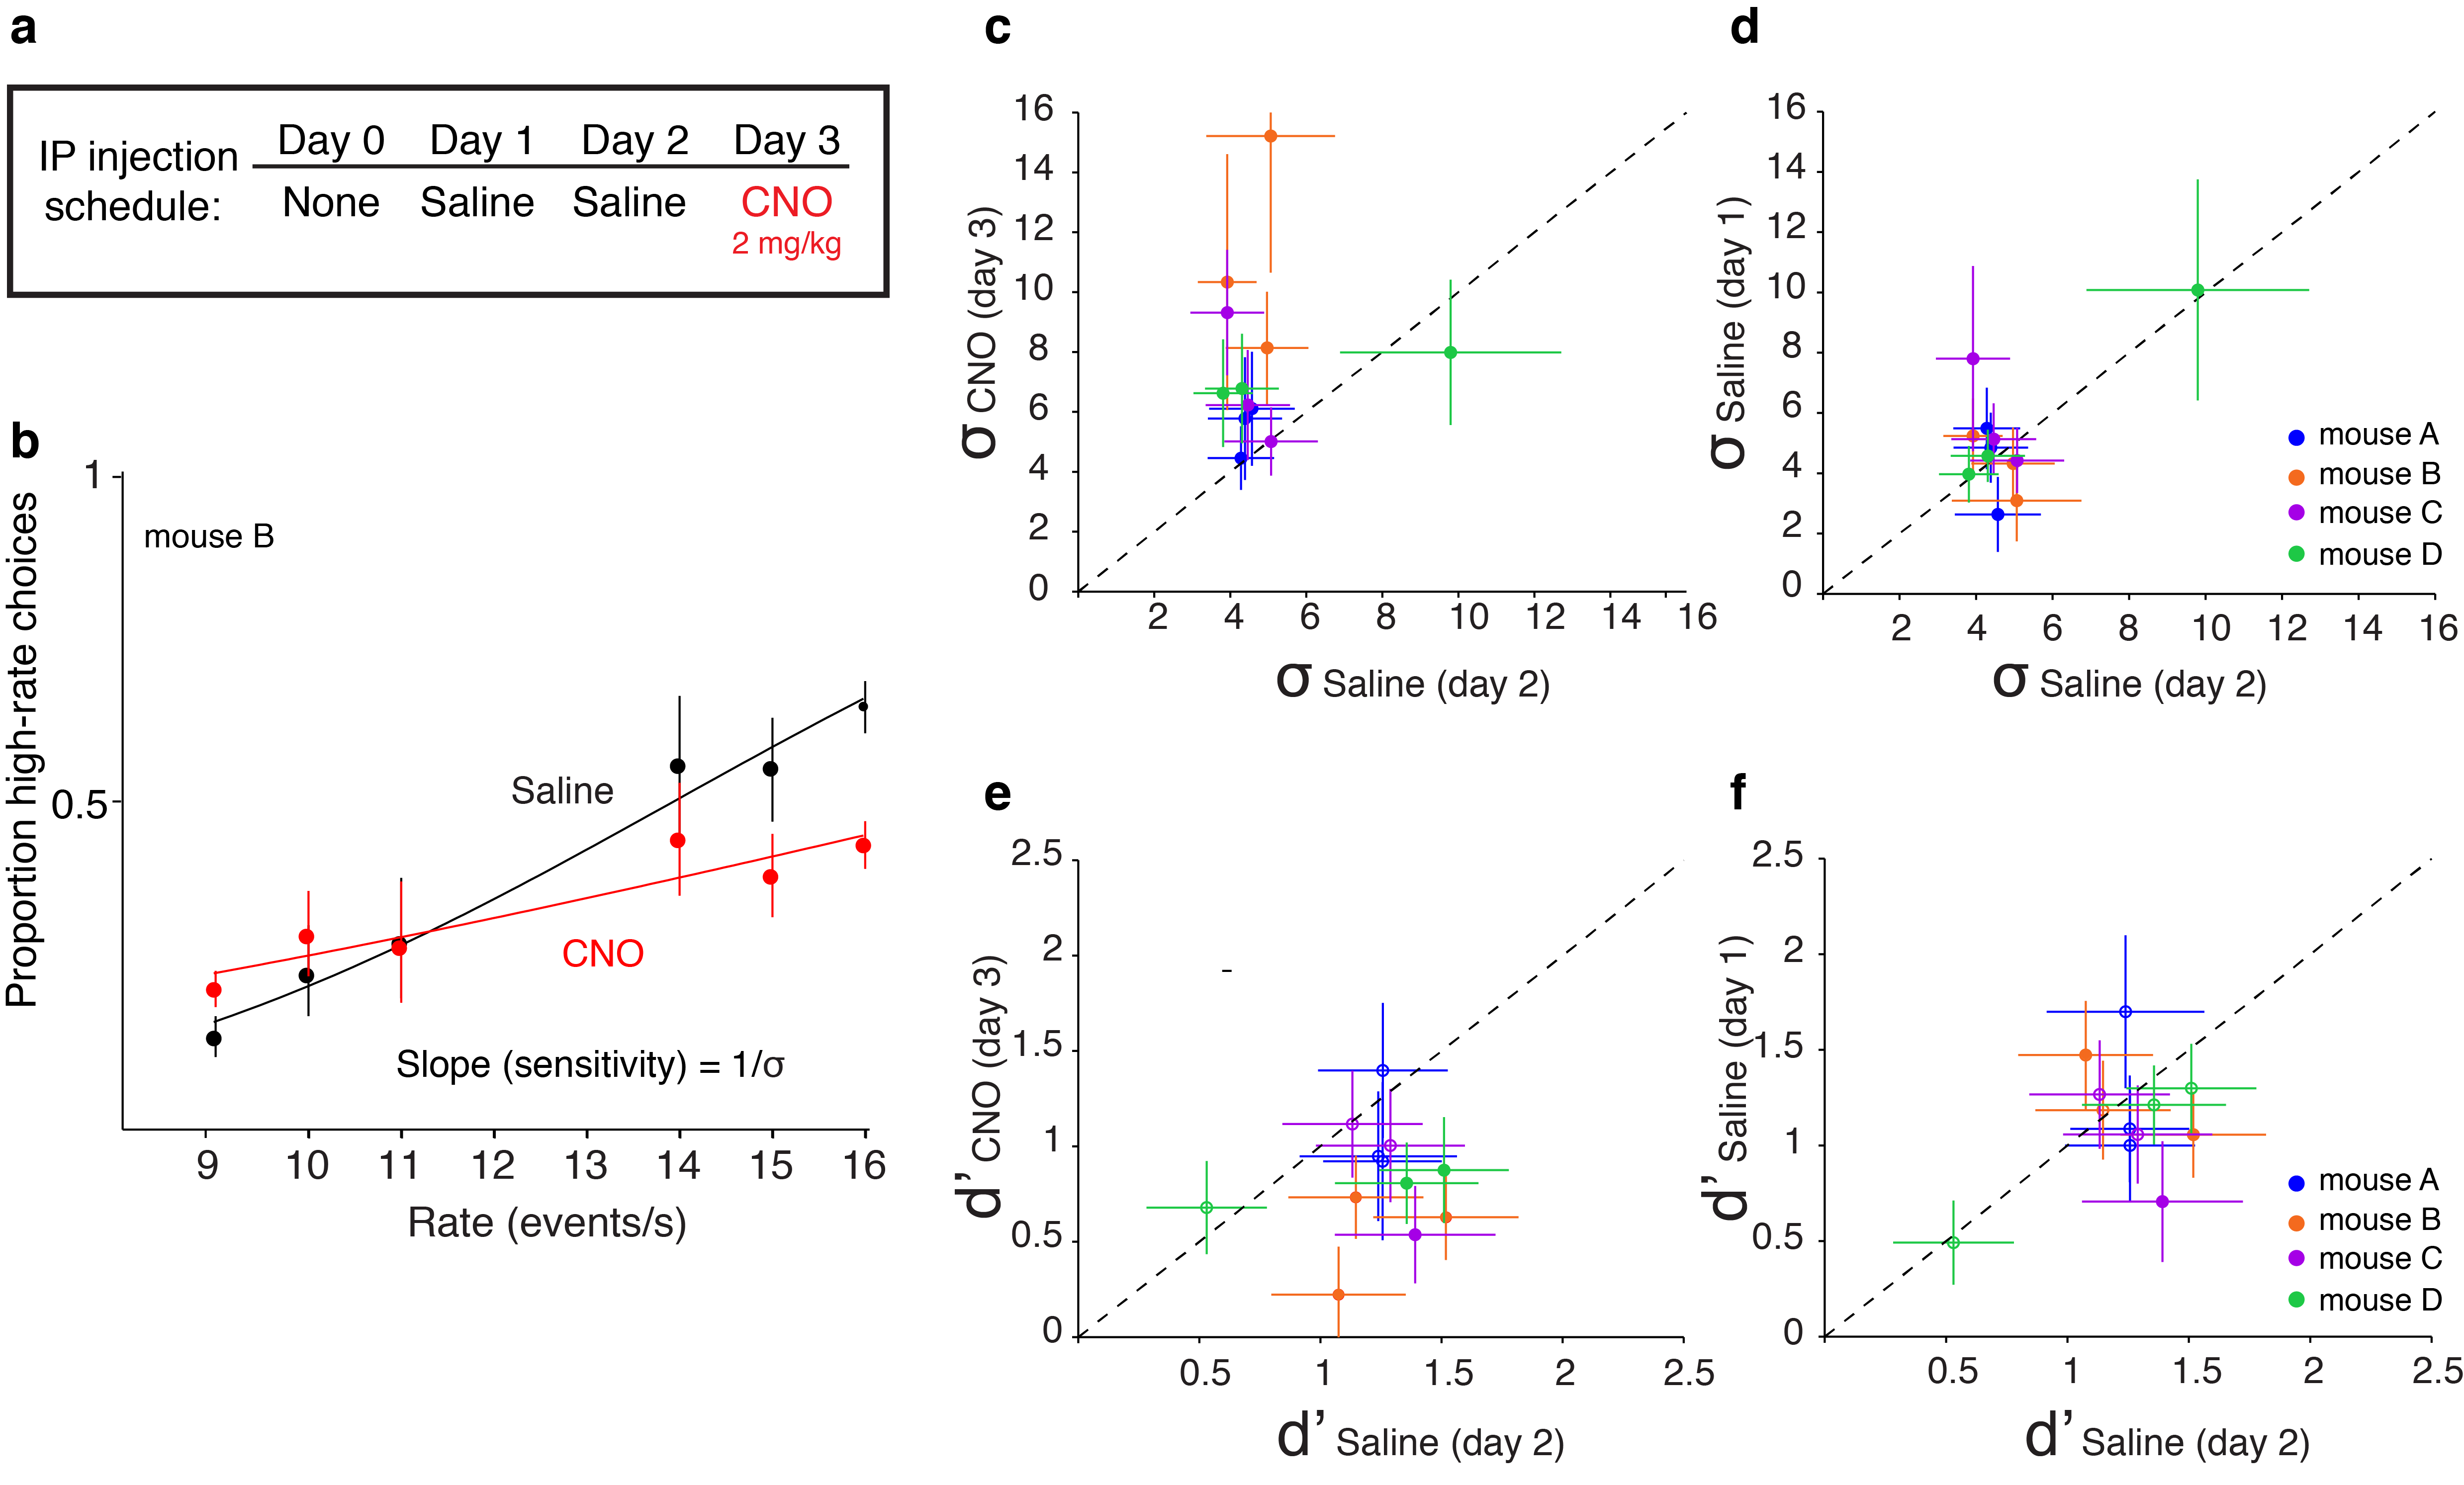
\includegraphics[width=\textwidth]{Figures/chapter3/psychophysics_dreadd_disruption.png}
  \caption[Chemogenetic silencing of mouse PPC disrupts psychophysical performance]{\textbf{Chemogenetic silencing of mouse PPC disrupts psychophysical performance.} (a) CNO and Saline treatment schedule. Saline typically administered two session prior to CNO treatment,(b) Mean psychometric performance of single mouse (n=3 CNO sessions, n= 3 saline sessions). (c) Summary of CNO vs. Saline control psychometric curve slope comparison (n=4 mice, 3 CNO/Saline sessions per mouse) shows performance impaired on CNO sessions compared to saline control sessions. (d) Summary comparison between two saline control days largely show no difference.(e) Comparison of d' on CNO vs saline control sessions also shows performance impairment on CNO sessions. (f) d' comparison of saline control sessions.}
  \label{fig:dreaddallmice}
\end{figure}
\begin{figure}
  \centering
  	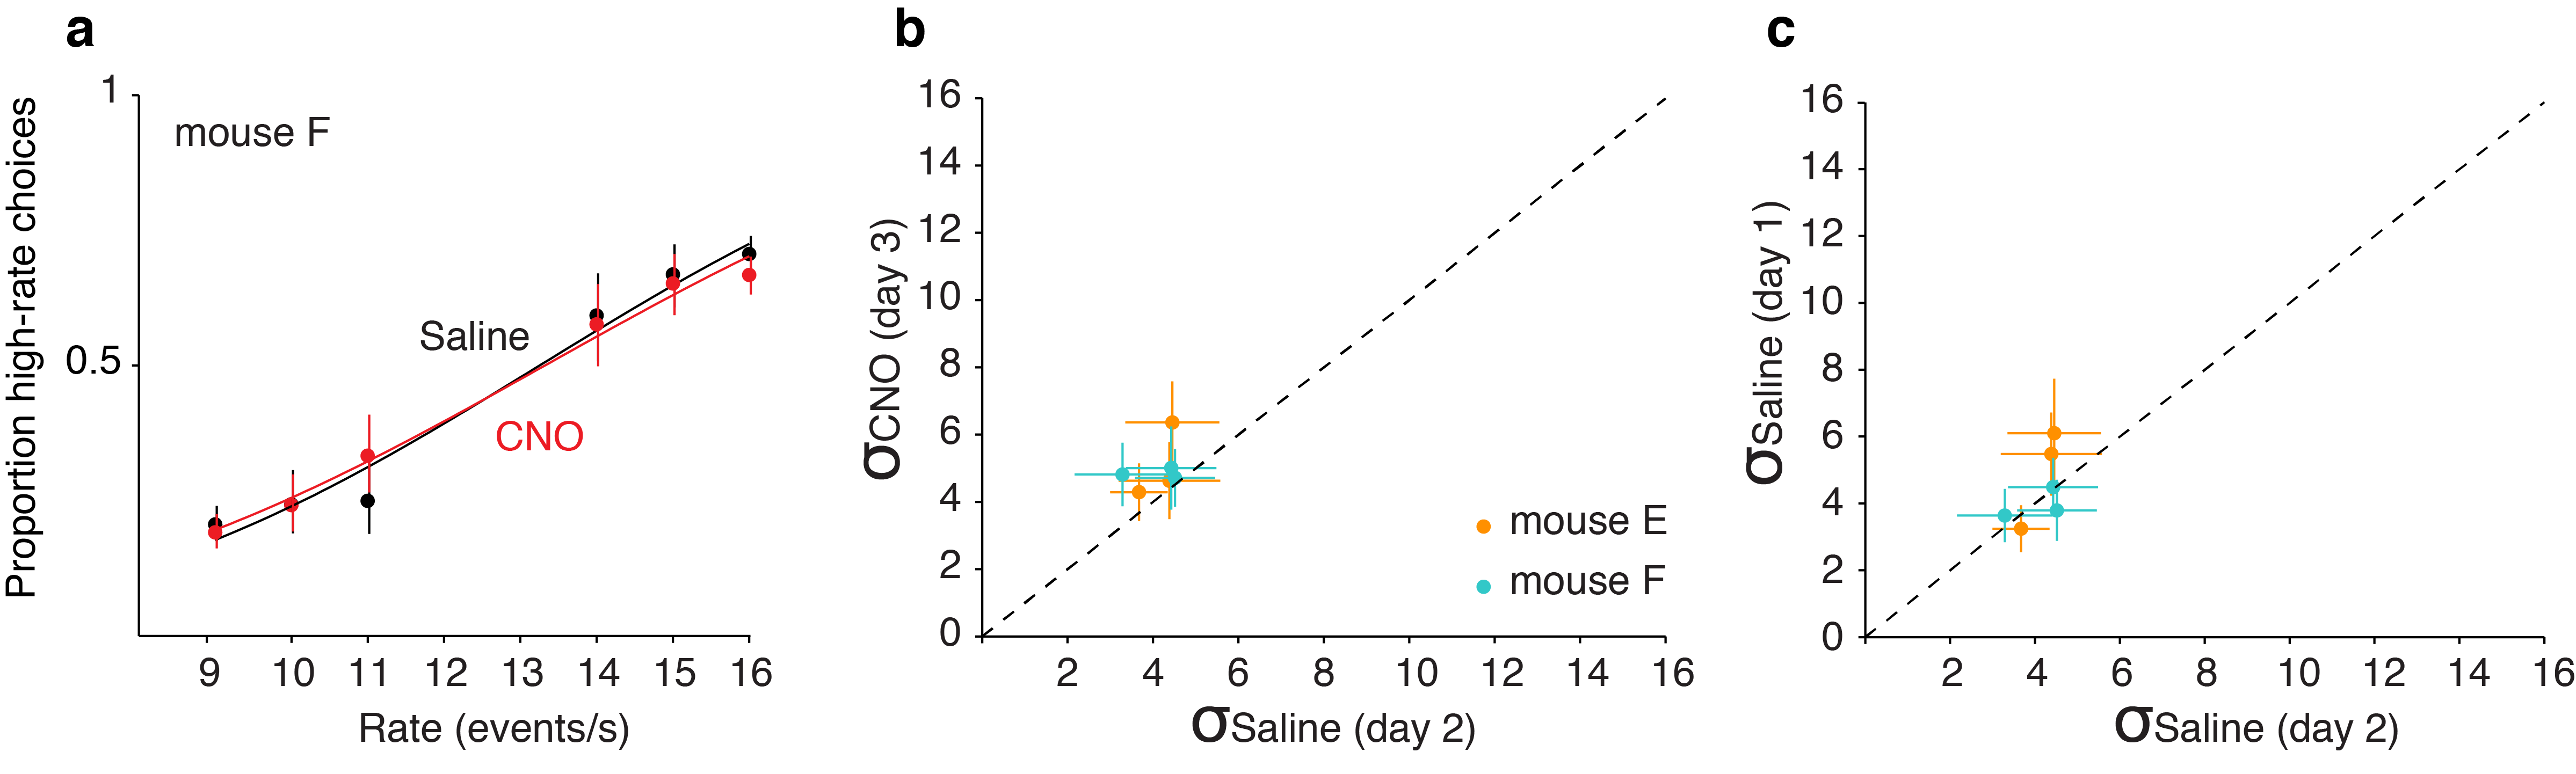
\includegraphics[width=\textwidth]{Figures/chapter3/dreadd_uninjected_control_mice.png}
  \caption[Uninjected DREADD virus control group]{\textbf{Uninjected DREADD virus control group.} CNO administration to wildtype animals did not affect decision-making accuracy. (a) Mean psychometric function of CNO-treated and saline treated sessions (n = 3 CNO/Saline sessions) for single mouse. Comparison of psychometric function slope (b) CNO- vs Saline-treated sessions, and (c) Saline vs. Saline-treated sessions.}
   \label{fig:dreaddcontrol}
\end{figure}
The disruption of psychophysical performance due to PPC DREADD manipulation could be explained by a number of factors. For instance, the behavioral impairment could be explained simply by the administration of CNO. To test this, I repeated the experiments in a cohort of wildtype mice (n = 2) that were not infected with DREADD receptor and observed no difference in psychophysical performance between CNO- and saline- treated sessions (Figure \ref{fig:dreaddcontrol}). Another plausible explanation for decreased psychophysical performance is that the mice failed to complete as many trials on CNO treatment sessions compared to saline sessions. However, mice completed just as many trials on CNO as on saline sessions and equally waited the minimum duration (1000 ms) before making a choice (Figure \ref{fig:dreaddtaskmeasures}a,b). However, the movement duration from the center port to the choice port was slightly slower on CNO treated sessions (Figure \ref{fig:dreaddtaskmeasures}c).\par 

\begin{figure}
  \centering
  	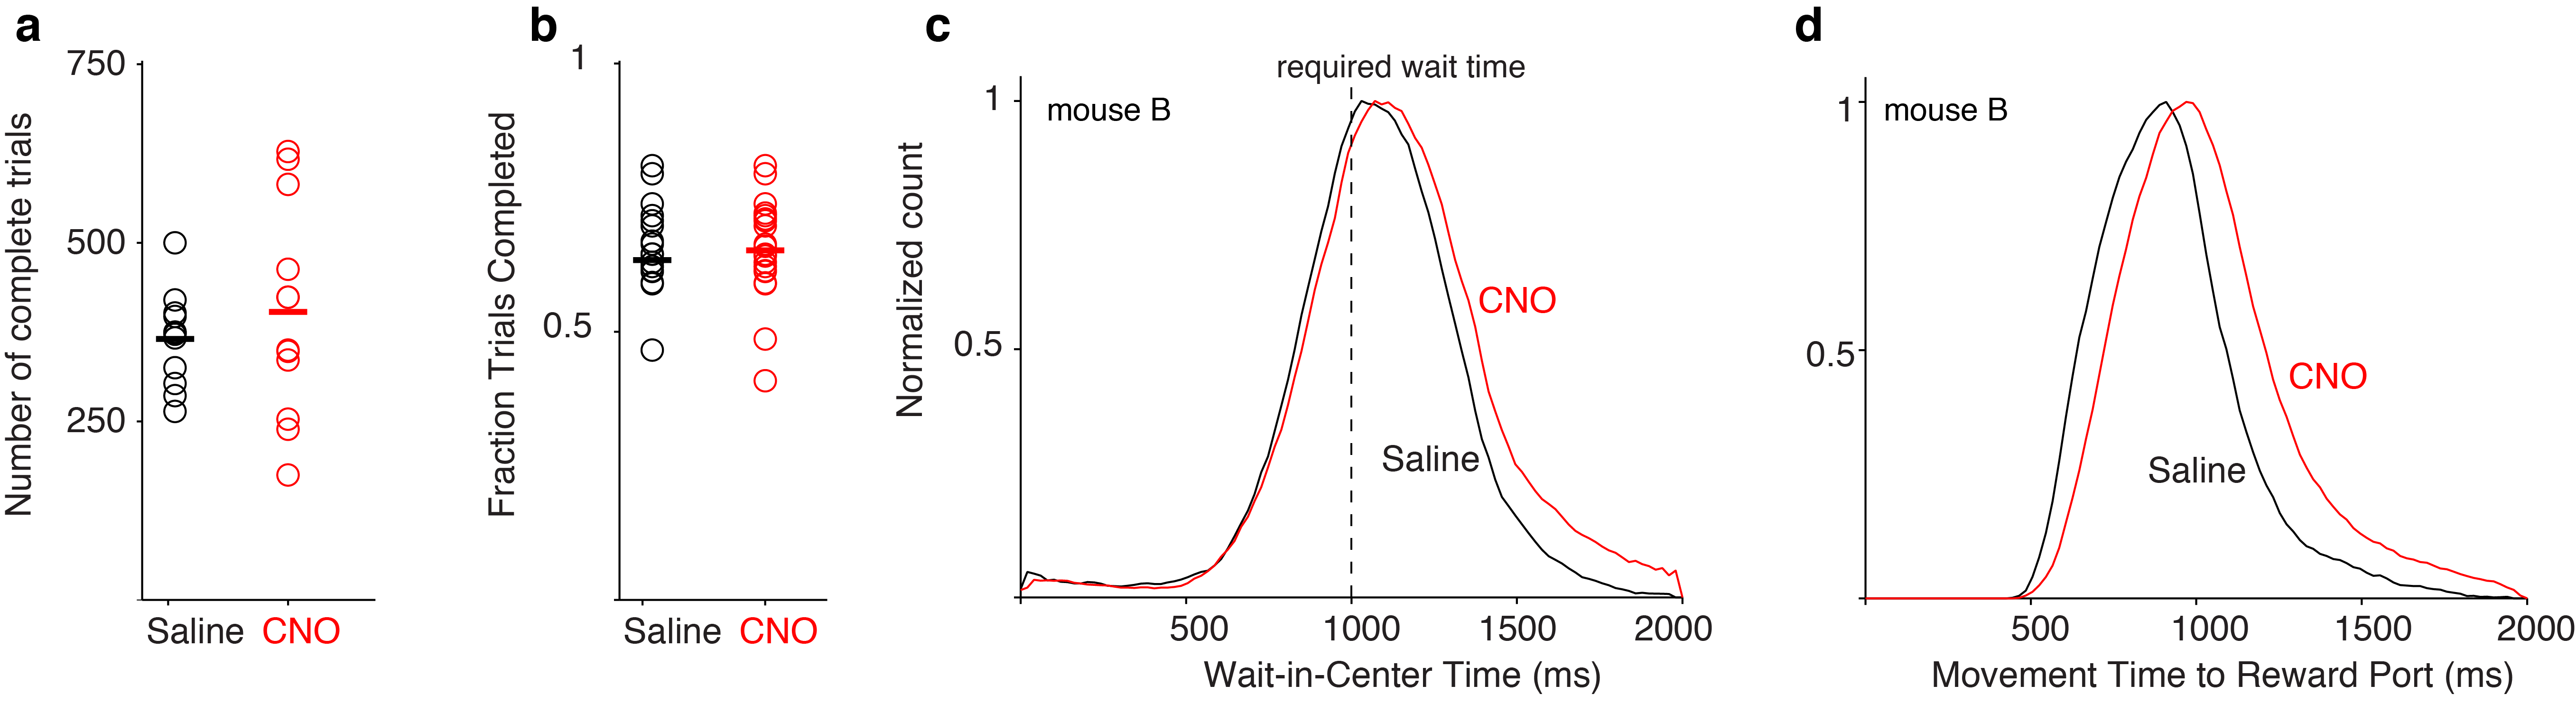
\includegraphics[width=\textwidth]{Figures/chapter3/non-stimulus_related_task_variables.png}
  \caption[Other task parameters unaffected by DREADD manipulation]{\textbf{Other task parameters unaffected by DREADD manipulation.} PPC manipulation  did not reduce the (a) number or (b) fraction of completed trials. (c) DREADD manipulation of PPC did not impair ability to wait the minimum required time before reporting choice. (d) PPC manipulation slightly increased movement duration to the reward port.}
   \label{fig:dreaddtaskmeasures}
\end{figure}
PPC DREADD manipulation could have differential effects during the course of a session. For example the CNO-induced DREADD perturbation could have a stronger effect early in the session, or conversely, it might take longer for the DREADD manipulation to take effect. To examine these potential scenarios, I compared the average percent correct performance across the first 200 trials (early) and the last 200 trials (late) (Figure \ref{fig:dreaddinsession}). Comparable decreases in performance were observed between early and late on CNO treated and saline control sessions.\par 
\begin{figure}
  \centering
  	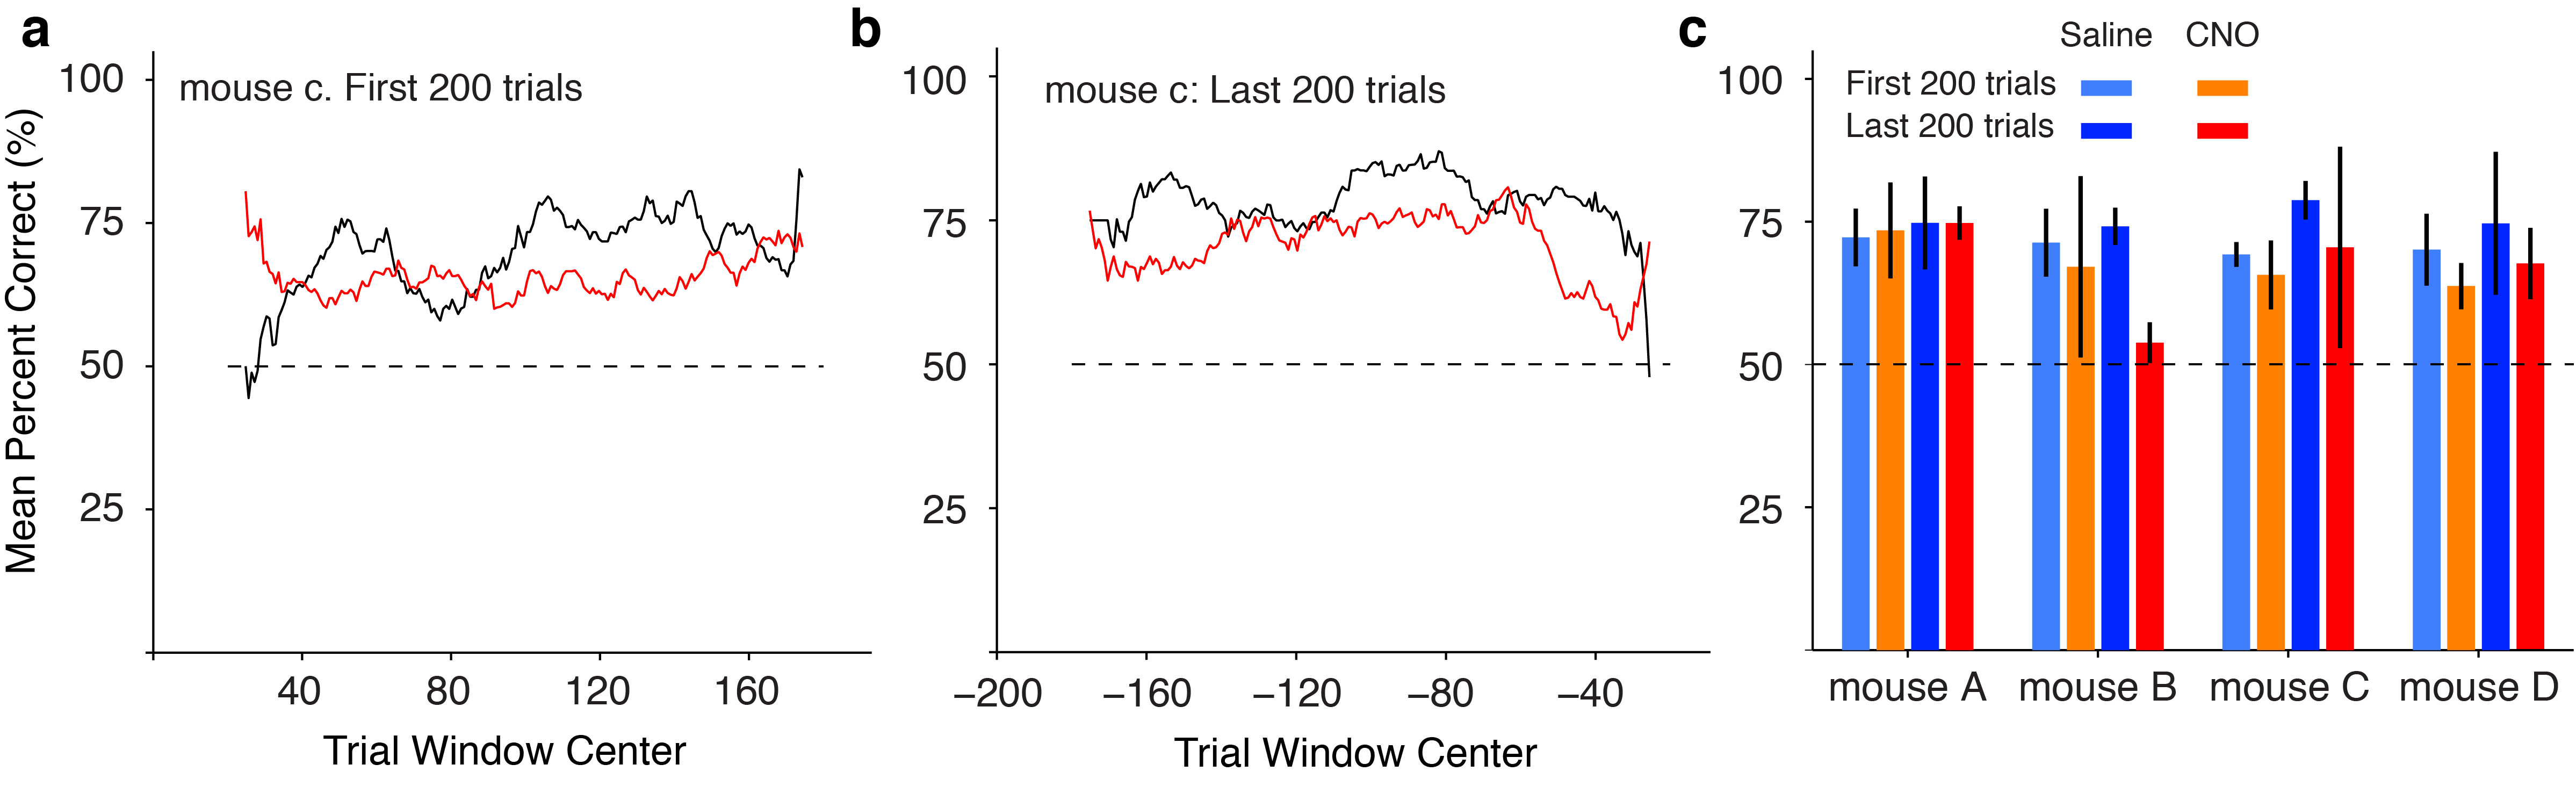
\includegraphics[width=\textwidth]{Figures/chapter3/within_session_comparison.png}
  \caption[Within session comparison of DREADD disruption]{\textbf{Within session comparison of DREADD disruption.} CNO treatment affected mean percent correct comparably for early and late in the session. Average percent correct across the (a) first 200 trials and (b) last 200 trials in session for single mouse. Black line represents control sessions. Red line represent CNO treatment sessions. (c) Average percent correct during first and last 200 trials for all mice.} 
   \label{fig:dreaddinsession}
\end{figure}
CNO is a reversible metabolite of the anti-psychotic drug, clozapine \parencite{Lin1994,Chang1998}. A potential concern was that higher doses and repeated exposure of the mice to CNO could have potential harmful and off target effects if CNO metabolized into clozapine. To evaluate the lifetime of CNO in the blood and to assess whether CNO metabolizes into clozapine, I collected blood serum from mice at different time points after CNO injection (Figure \ref{fig:dreaddcnoblood}). The blood serum was analyzed with mass spectroscopy at the CSHL Proteomics core facility. CNO clears the blood efficiently, in less than 20 minutes. There is also very minimal conversion of the CNO to clozapine. Our observation is consistent with a recent study \parencite{Guettier2009} that reported negligible conversion of CNO to clozapine. However, it is not clear how well the concentration of CNO in the blood relates to the amount of CNO (and/or clozapine) that enters the brain. 
\begin{figure}
  \centering
  	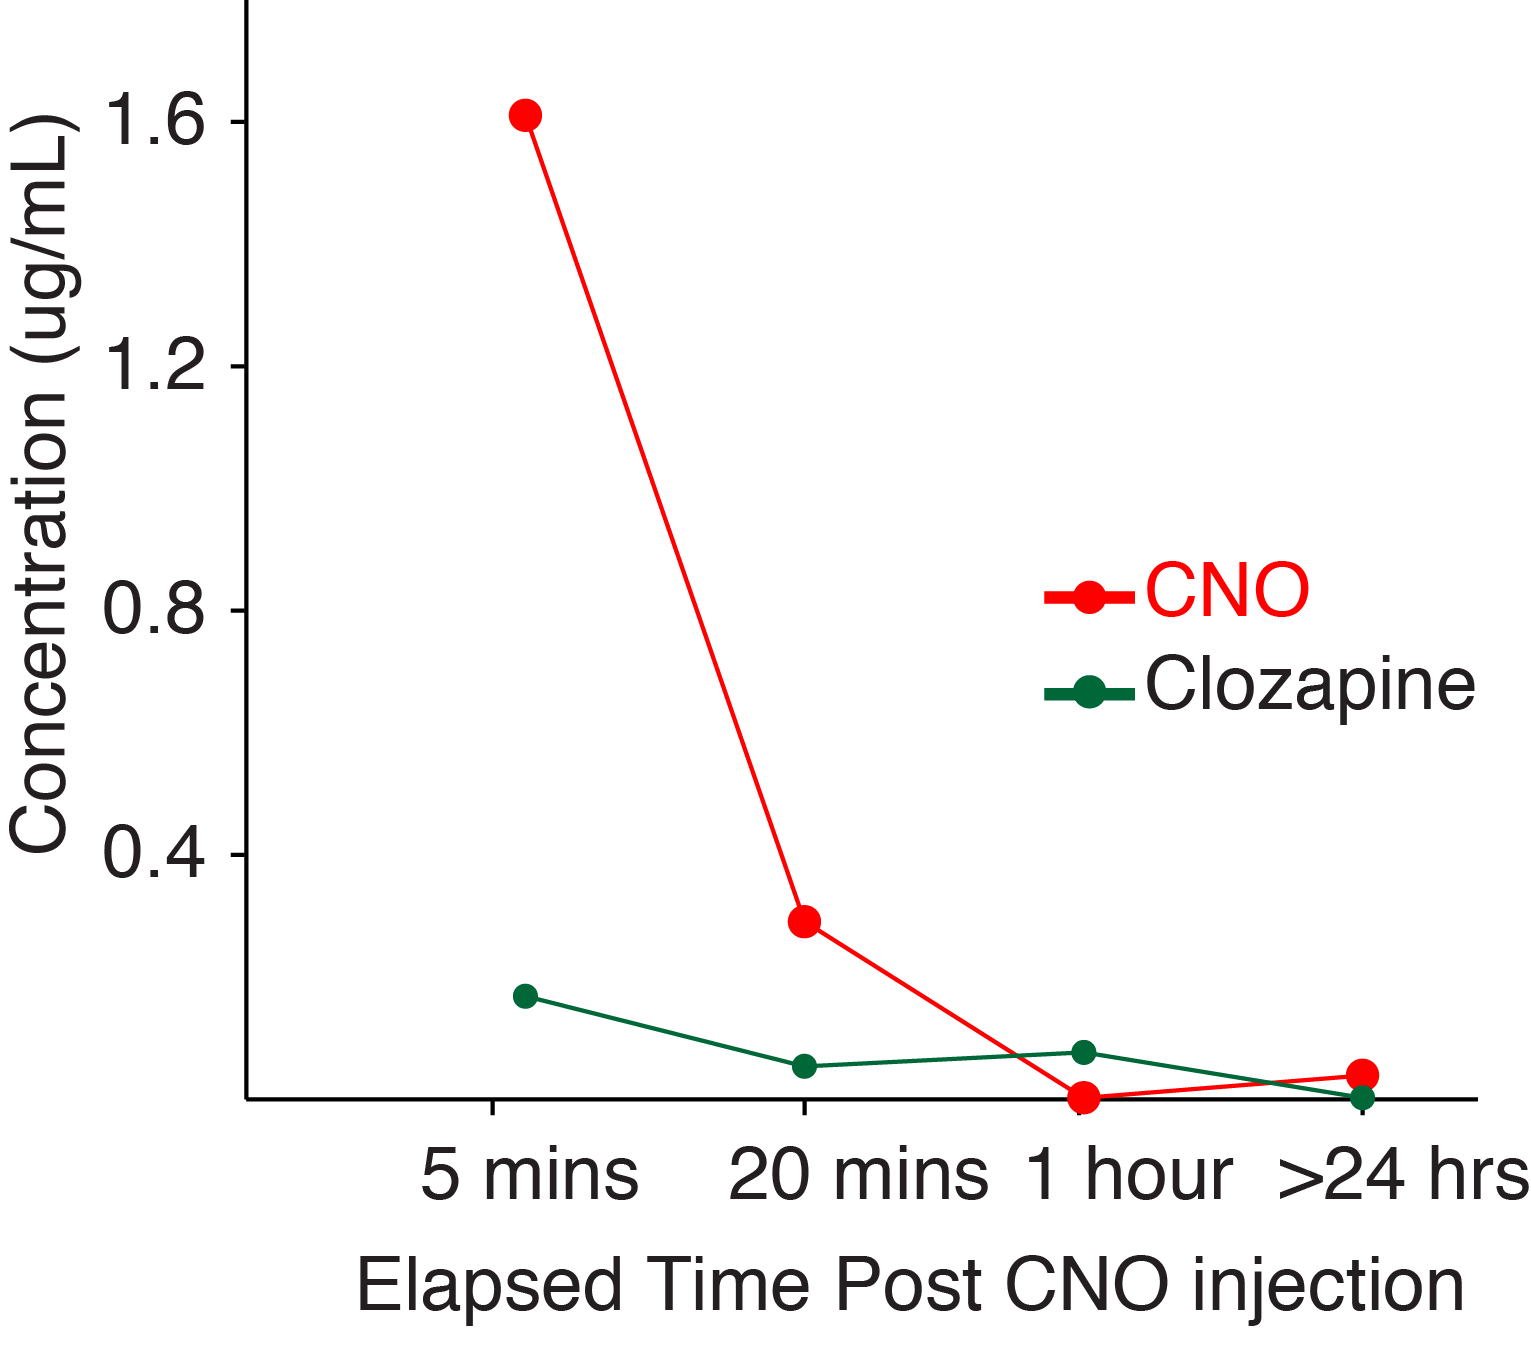
\includegraphics[scale=0.5]{Figures/chapter3/cno_lifetime_in_the_blood.png}
  \caption[CNO Lifetime in Blood Plasma]{\textbf{CNO Lifetime in Blood Plasma.} from an example mouse. CNO in the blood plasma rapidly decreases after IP injection.}
   \label{fig:dreaddcnoblood}
\end{figure}
\section{Discussion}
This chapter demonstrated that reversible chemogenetic disruption of mouse PPC by inhibition of inhibitory neurons reduced psychophysical performance. The result provides evidence that cortical machinery, in mice, plays a causal role in our visual evidence accumulation task. Chemogenetic disruption of mouse PPC did not impair the subjects' ability to execute the task, although the movement response time to the reward port was modestly reduced. In addition, control animals were not affected by CNO treatment in the absence of the DREADD receptor.\par 
The choice for PPC disruption was inspired by computational frameworks of perceptual decision making which highlight the role of inhibitory neurons in the neural implementation of the decision process \parencite{Beck2008,Wang2002}. Silencing inhibitory neurons is equivalent to adding aberrant noise to the circuit or tipping the cortical balance of excitation and inhibition (E/I balance) towards excitation. Inhibition is essential to shaping cortical computations \parencite{Haider2006,Haider2012,Isaacson2011}, and interfering with cortical balance of excitation-to-inhibition impacts local and global network activity and may underlie cognitive deficits \parencite{Markram2010,Rubenstein2010,Rubenstein2003,Yizhar2011}. Though simultaneous electrophysiological recordings were not performed to confirm the true nature of our chemogenetic PPC disruption, I speculate that the net effect on the circuit is increased local excitatory activity within PPC. If this is the case, the behavioral deficits observed in the mice are consistent with recent results from the Churchland lab \parencite{Licata2017}, which used an optogenetic strategy to directly elevate activity in rat PPC. In the \textcite{Licata2017} study, artificial excitatory drive in rat PPC also impaired accuracy on visual decisions, but had no effect on auditory decisions. These similar findings suggest a potentially conserved role for rodent PPC involvement in the process of evidence accumulation of visual decision making. 



